\documentclass{extbook}[14pt]
\usepackage{multicol, enumerate, enumitem, hyperref, color, soul, setspace, parskip, fancyhdr, amssymb, amsthm, amsmath, latexsym, units, mathtools}
\everymath{\displaystyle}
\usepackage[headsep=0.5cm,headheight=0cm, left=1 in,right= 1 in,top= 1 in,bottom= 1 in]{geometry}
\usepackage{dashrule}  % Package to use the command below to create lines between items
\newcommand{\litem}[1]{\item #1

\rule{\textwidth}{0.4pt}}
\pagestyle{fancy}
\lhead{}
\chead{Answer Key for Progress Quiz 6 Version B}
\rhead{}
\lfoot{9689-6866}
\cfoot{}
\rfoot{Spring 2021}
\begin{document}
\textbf{This key should allow you to understand why you choose the option you did (beyond just getting a question right or wrong). \href{https://xronos.clas.ufl.edu/mac1105spring2020/courseDescriptionAndMisc/Exams/LearningFromResults}{More instructions on how to use this key can be found here}.}

\textbf{If you have a suggestion to make the keys better, \href{https://forms.gle/CZkbZmPbC9XALEE88}{please fill out the short survey here}.}

\textit{Note: This key is auto-generated and may contain issues and/or errors. The keys are reviewed after each exam to ensure grading is done accurately. If there are issues (like duplicate options), they are noted in the offline gradebook. The keys are a work-in-progress to give students as many resources to improve as possible.}

\rule{\textwidth}{0.4pt}

\begin{enumerate}\litem{
Construct the lowest-degree polynomial given the zeros below. Then, choose the intervals that contain the coefficients of the polynomial in the form $ax^3+bx^2+cx+d$.
\[ \frac{5}{2}, 4, \text{ and } \frac{7}{2} \]The solution is \( 4x^{3} -40 x^{2} +131 x -140 \), which is option E.\begin{enumerate}[label=\Alph*.]
\item \( a \in [-1, 6], b \in [36, 45], c \in [129, 132], \text{ and } d \in [133, 144] \)

$4x^{3} +40 x^{2} +131 x + 140$, which corresponds to multiplying out $(2x + 5)(x + 4)(2x + 7)$.
\item \( a \in [-1, 6], b \in [7, 14], c \in [-52, -45], \text{ and } d \in [-143, -137] \)

$4x^{3} +12 x^{2} -51 x -140$, which corresponds to multiplying out $(2x + 5)(x + 4)(2x -7)$.
\item \( a \in [-1, 6], b \in [-48, -32], c \in [129, 132], \text{ and } d \in [133, 144] \)

$4x^{3} -40 x^{2} +131 x + 140$, which corresponds to multiplying everything correctly except the constant term.
\item \( a \in [-1, 6], b \in [-26, -19], c \in [-27, -17], \text{ and } d \in [133, 144] \)

$4x^{3} -20 x^{2} -19 x + 140$, which corresponds to multiplying out $(2x + 5)(x -4)(2x -7)$.
\item \( a \in [-1, 6], b \in [-48, -32], c \in [129, 132], \text{ and } d \in [-143, -137] \)

* $4x^{3} -40 x^{2} +131 x -140$, which is the correct option.
\end{enumerate}

\textbf{General Comment:} To construct the lowest-degree polynomial, you want to multiply out $(2x -5)(x -4)(2x -7)$
}
\litem{
Describe the zero behavior of the zero $x = 9$ of the polynomial below.
\[ f(x) = 7(x + 8)^{8}(x - 8)^{7}(x + 9)^{12}(x - 9)^{7} \]The solution is the graph below, which is option D.
\begin{center}
    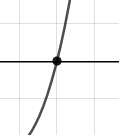
\includegraphics[width=0.3\textwidth]{../Figures/polyZeroBehaviorDB.png}
\end{center}\begin{enumerate}[label=\Alph*.]
\begin{multicols}{2}
\item 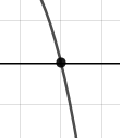
\includegraphics[width = 0.3\textwidth]{../Figures/polyZeroBehaviorAB.png}
\item 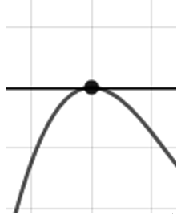
\includegraphics[width = 0.3\textwidth]{../Figures/polyZeroBehaviorBB.png}
\item 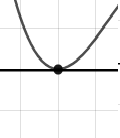
\includegraphics[width = 0.3\textwidth]{../Figures/polyZeroBehaviorCB.png}
\item 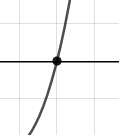
\includegraphics[width = 0.3\textwidth]{../Figures/polyZeroBehaviorDB.png}
\end{multicols}\item None of the above.\end{enumerate}
\textbf{General Comment:} You will need to sketch the entire graph, then zoom in on the zero the question asks about.
}
\litem{
Which of the following equations \textit{could} be of the graph presented below?

\begin{center}
    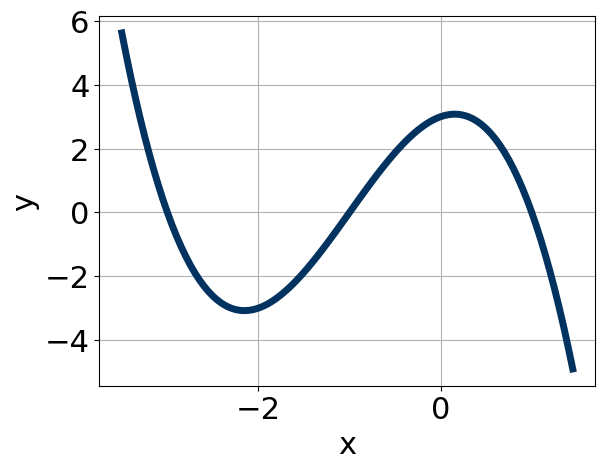
\includegraphics[width=0.5\textwidth]{../Figures/polyGraphToFunctionB.png}
\end{center}


The solution is \( 6(x - 3)^{6} (x + 3)^{8} (x - 2)^{8} \), which is option D.\begin{enumerate}[label=\Alph*.]
\item \( -4(x - 3)^{6} (x + 3)^{8} (x - 2)^{7} \)

The factor $(x - 2)$ should have an even power and the leading coefficient should be the opposite sign.
\item \( -11(x - 3)^{4} (x + 3)^{10} (x - 2)^{8} \)

This corresponds to the leading coefficient being the opposite value than it should be.
\item \( 6(x - 3)^{4} (x + 3)^{9} (x - 2)^{9} \)

The factors $(x + 3)$ and $(x - 2)$ should both have even powers.
\item \( 6(x - 3)^{6} (x + 3)^{8} (x - 2)^{8} \)

* This is the correct option.
\item \( 19(x - 3)^{8} (x + 3)^{10} (x - 2)^{7} \)

The factor $(x - 2)$ should have an even power.
\end{enumerate}

\textbf{General Comment:} General Comments: Draw the x-axis to determine which zeros are touching (and so have even multiplicity) or cross (and have odd multiplicity).
}
\litem{
Describe the zero behavior of the zero $x = 9$ of the polynomial below.
\[ f(x) = -4(x + 9)^{9}(x - 9)^{10}(x - 2)^{7}(x + 2)^{10} \]The solution is the graph below, which is option B.
\begin{center}
    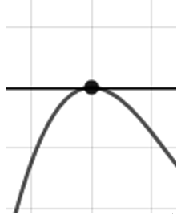
\includegraphics[width=0.3\textwidth]{../Figures/polyZeroBehaviorCopyBB.png}
\end{center}\begin{enumerate}[label=\Alph*.]
\begin{multicols}{2}
\item 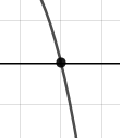
\includegraphics[width = 0.3\textwidth]{../Figures/polyZeroBehaviorCopyAB.png}
\item 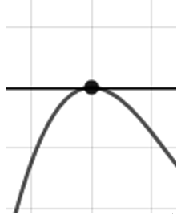
\includegraphics[width = 0.3\textwidth]{../Figures/polyZeroBehaviorCopyBB.png}
\item 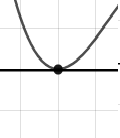
\includegraphics[width = 0.3\textwidth]{../Figures/polyZeroBehaviorCopyCB.png}
\item 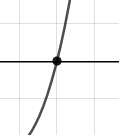
\includegraphics[width = 0.3\textwidth]{../Figures/polyZeroBehaviorCopyDB.png}
\end{multicols}\item None of the above.\end{enumerate}
\textbf{General Comment:} You will need to sketch the entire graph, then zoom in on the zero the question asks about.
}
\litem{
Which of the following equations \textit{could} be of the graph presented below?

\begin{center}
    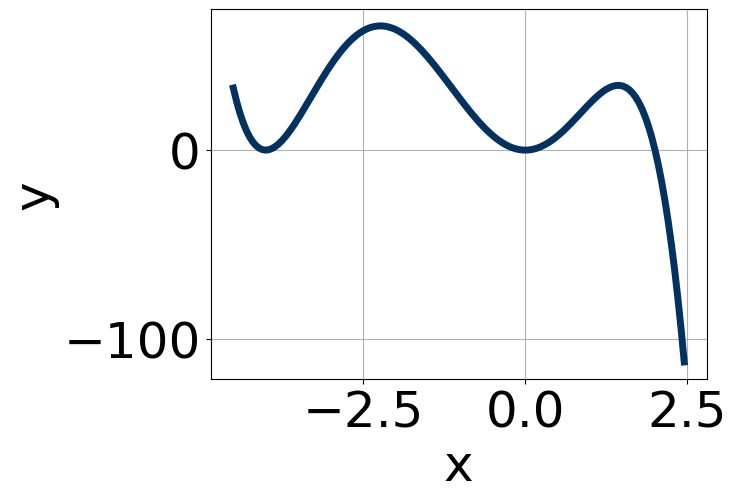
\includegraphics[width=0.5\textwidth]{../Figures/polyGraphToFunctionCopyB.png}
\end{center}


The solution is \( 12x^{11} (x - 2)^{11} (x - 1)^{11} \), which is option E.\begin{enumerate}[label=\Alph*.]
\item \( -12x^{9} (x - 2)^{5} (x - 1)^{11} \)

This corresponds to the leading coefficient being the opposite value than it should be.
\item \( 18x^{4} (x - 2)^{6} (x - 1)^{11} \)

The factors $0$ and $2$ have have been odd power.
\item \( 10x^{10} (x - 2)^{5} (x - 1)^{11} \)

The factor $0$ should have been an odd power.
\item \( -10x^{6} (x - 2)^{11} (x - 1)^{9} \)

The factor $x$ should have an odd power and the leading coefficient should be the opposite sign.
\item \( 12x^{11} (x - 2)^{11} (x - 1)^{11} \)

* This is the correct option.
\end{enumerate}

\textbf{General Comment:} General Comments: Draw the x-axis to determine which zeros are touching (and so have even multiplicity) or cross (and have odd multiplicity).
}
\litem{
Describe the end behavior of the polynomial below.
\[ f(x) = -9(x + 9)^{2}(x - 9)^{3}(x + 7)^{2}(x - 7)^{2} \]The solution is the graph below, which is option A.
\begin{center}
    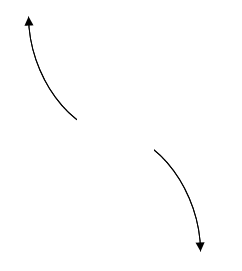
\includegraphics[width=0.3\textwidth]{../Figures/polyEndBehaviorCopyAB.png}
\end{center}\begin{enumerate}[label=\Alph*.]
\begin{multicols}{2}
\item 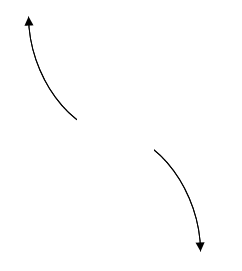
\includegraphics[width = 0.3\textwidth]{../Figures/polyEndBehaviorCopyAB.png}
\item 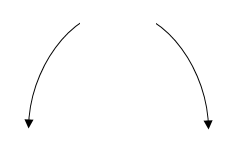
\includegraphics[width = 0.3\textwidth]{../Figures/polyEndBehaviorCopyBB.png}
\item 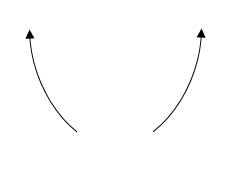
\includegraphics[width = 0.3\textwidth]{../Figures/polyEndBehaviorCopyCB.png}
\item 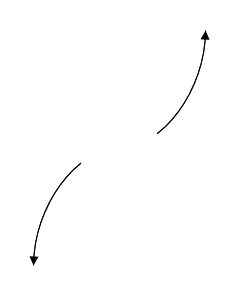
\includegraphics[width = 0.3\textwidth]{../Figures/polyEndBehaviorCopyDB.png}
\end{multicols}\item None of the above.\end{enumerate}
\textbf{General Comment:} Remember that end behavior is determined by the leading coefficient AND whether the \textbf{sum} of the multiplicities is positive or negative.
}
\litem{
Construct the lowest-degree polynomial given the zeros below. Then, choose the intervals that contain the coefficients of the polynomial in the form $x^3+bx^2+cx+d$.
\[ -3 - 5 i \text{ and } 1 \]The solution is \( x^{3} +5 x^{2} +28 x -34 \), which is option C.\begin{enumerate}[label=\Alph*.]
\item \( b \in [-6.1, -3.5], c \in [26.18, 29.01], \text{ and } d \in [32.07, 34.51] \)

$x^{3} -5 x^{2} +28 x + 34$, which corresponds to multiplying out $(x-(-3 - 5 i))(x-(-3 + 5 i))(x + 1)$.
\item \( b \in [0.1, 4.8], c \in [0.84, 2.43], \text{ and } d \in [-3.52, -2.55] \)

$x^{3} + x^{2} +2 x -3$, which corresponds to multiplying out $(x + 3)(x -1)$.
\item \( b \in [3.2, 10.8], c \in [26.18, 29.01], \text{ and } d \in [-35.08, -33.01] \)

* $x^{3} +5 x^{2} +28 x -34$, which is the correct option.
\item \( b \in [0.1, 4.8], c \in [3.67, 5.55], \text{ and } d \in [-5.68, -3.99] \)

$x^{3} + x^{2} +4 x -5$, which corresponds to multiplying out $(x + 5)(x -1)$.
\item \( \text{None of the above.} \)

This corresponds to making an unanticipated error or not understanding how to use nonreal complex numbers to create the lowest-degree polynomial. If you chose this and are not sure what you did wrong, please contact the coordinator for help.
\end{enumerate}

\textbf{General Comment:} Remember that the conjugate of $a+bi$ is $a-bi$. Since these zeros always come in pairs, we need to multiply out $(x-(-3 - 5 i))(x-(-3 + 5 i))(x-(1))$.
}
\litem{
Describe the end behavior of the polynomial below.
\[ f(x) = 3(x - 6)^{4}(x + 6)^{7}(x - 5)^{2}(x + 5)^{2} \]The solution is the graph below, which is option D.
\begin{center}
    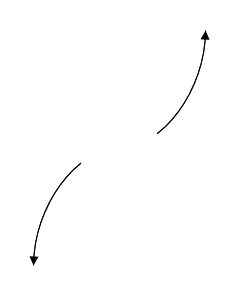
\includegraphics[width=0.3\textwidth]{../Figures/polyEndBehaviorDB.png}
\end{center}\begin{enumerate}[label=\Alph*.]
\begin{multicols}{2}
\item 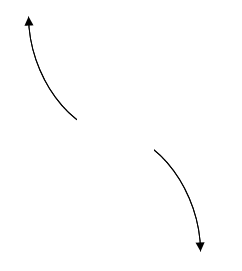
\includegraphics[width = 0.3\textwidth]{../Figures/polyEndBehaviorAB.png}
\item 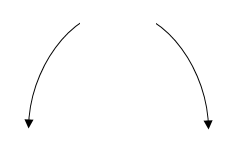
\includegraphics[width = 0.3\textwidth]{../Figures/polyEndBehaviorBB.png}
\item 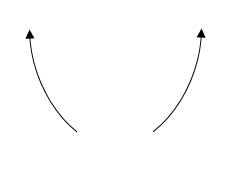
\includegraphics[width = 0.3\textwidth]{../Figures/polyEndBehaviorCB.png}
\item 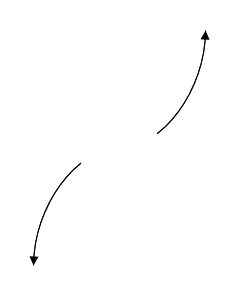
\includegraphics[width = 0.3\textwidth]{../Figures/polyEndBehaviorDB.png}
\end{multicols}\item None of the above.\end{enumerate}
\textbf{General Comment:} Remember that end behavior is determined by the leading coefficient AND whether the \textbf{sum} of the multiplicities is positive or negative.
}
\litem{
Construct the lowest-degree polynomial given the zeros below. Then, choose the intervals that contain the coefficients of the polynomial in the form $x^3+bx^2+cx+d$.
\[ 4 - 4 i \text{ and } 1 \]The solution is \( x^{3} -9 x^{2} +40 x -32 \), which is option C.\begin{enumerate}[label=\Alph*.]
\item \( b \in [5, 10], c \in [31, 46], \text{ and } d \in [24, 34] \)

$x^{3} +9 x^{2} +40 x + 32$, which corresponds to multiplying out $(x-(4 - 4 i))(x-(4 + 4 i))(x + 1)$.
\item \( b \in [1, 2], c \in [-10, -1], \text{ and } d \in [3, 12] \)

$x^{3} + x^{2} -5 x + 4$, which corresponds to multiplying out $(x -4)(x -1)$.
\item \( b \in [-14, -8], c \in [31, 46], \text{ and } d \in [-34, -30] \)

* $x^{3} -9 x^{2} +40 x -32$, which is the correct option.
\item \( b \in [1, 2], c \in [3, 4], \text{ and } d \in [-5, 0] \)

$x^{3} + x^{2} +3 x -4$, which corresponds to multiplying out $(x + 4)(x -1)$.
\item \( \text{None of the above.} \)

This corresponds to making an unanticipated error or not understanding how to use nonreal complex numbers to create the lowest-degree polynomial. If you chose this and are not sure what you did wrong, please contact the coordinator for help.
\end{enumerate}

\textbf{General Comment:} Remember that the conjugate of $a+bi$ is $a-bi$. Since these zeros always come in pairs, we need to multiply out $(x-(4 - 4 i))(x-(4 + 4 i))(x-(1))$.
}
\litem{
Construct the lowest-degree polynomial given the zeros below. Then, choose the intervals that contain the coefficients of the polynomial in the form $ax^3+bx^2+cx+d$.
\[ \frac{1}{4}, -5, \text{ and } \frac{-7}{5} \]The solution is \( 20x^{3} +123 x^{2} +108 x -35 \), which is option D.\begin{enumerate}[label=\Alph*.]
\item \( a \in [17, 24], b \in [-128, -121], c \in [108, 114], \text{ and } d \in [32, 38] \)

$20x^{3} -123 x^{2} +108 x + 35$, which corresponds to multiplying out $(4x + 1)(x -5)(5x -7)$.
\item \( a \in [17, 24], b \in [132, 140], c \in [166, 173], \text{ and } d \in [32, 38] \)

$20x^{3} +133 x^{2} +172 x + 35$, which corresponds to multiplying out $(4x + 1)(x + 5)(5x + 7)$.
\item \( a \in [17, 24], b \in [118, 125], c \in [108, 114], \text{ and } d \in [32, 38] \)

$20x^{3} +123 x^{2} +108 x + 35$, which corresponds to multiplying everything correctly except the constant term.
\item \( a \in [17, 24], b \in [118, 125], c \in [108, 114], \text{ and } d \in [-42, -31] \)

* $20x^{3} +123 x^{2} +108 x -35$, which is the correct option.
\item \( a \in [17, 24], b \in [-70, -65], c \in [-163, -155], \text{ and } d \in [-42, -31] \)

$20x^{3} -67 x^{2} -158 x -35$, which corresponds to multiplying out $(4x + 1)(x -5)(5x + 7)$.
\end{enumerate}

\textbf{General Comment:} To construct the lowest-degree polynomial, you want to multiply out $(4x -1)(x + 5)(5x + 7)$
}
\end{enumerate}

\end{document}